% 유형 01 0039(본책 12쪽) — 직각삼각형 ABC(∠B=90°), AB=2 · BC=√5. 스캔 삽화를 TikZ 로 다시 그림.
% 라벨은 원문 그대로(2 · √5 · 꼭짓점 · 직각 표시). AC 의 길이(답의 근거)는 적지 않는다.
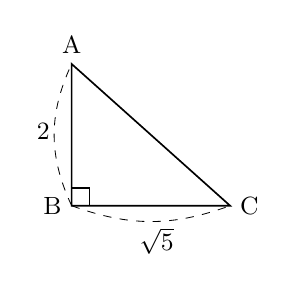
\begin{tikzpicture}[scale=0.9, line width=0.6pt]
  \coordinate (B) at (0,0); \coordinate (A) at (0,2); \coordinate (C) at (2.236,0);
  \draw (A) -- (B) -- (C) -- cycle;
  \draw[line width=0.4pt] (0,0.25) -- (0.25,0.25) -- (0.25,0);
  \draw[dashed, line width=0.3pt] (B) to[bend left=25] (A);
  \draw[dashed, line width=0.3pt] (B) to[bend right=20] (C);
  \node[font=\small, above] at (A) {A};
  \node[font=\small, left] at (B) {B};
  \node[font=\small, right] at (C) {C};
  \node[font=\small] at (-0.4,1.05) {$2$};
  \node[font=\small] at (1.2,-0.5) {$\sqrt{5}$};
\end{tikzpicture}
